\subsection{Primary submodules}

PROPOSITION 1. Let A be a Noetherian ring and M an A-module. The following conditions are equivalent: (a) Ass(M) is reduced to a single element.

\begin{enumerate}
\def\labelenumi{(\alph{enumi})}
\setcounter{enumi}{1}
\tightlist
\item
  \(\mathbf{M} \neq 0\) and every homothety of \(\mathbf{M}\) is either injective or almost nilpotent (§ 1, no. 4). If these conditions are fulfilled and \(\mathfrak{p}\) is the set of \(a \in \mathbf{A}\) such that the homothety \(a_{\mathbf{M}}\) is almost nilpotent, then \(\operatorname{Ass}(\mathbf{M}) = \{\mathfrak{p}\}\) .
\end{enumerate}

This follows immediately from § 1, no. 4, Corollary to Proposition 9 and no. 1, Corollary 2 to Proposition 2.

DEFINITION 1. Let A be a Noetherian ring, N an A-module and Q a submodule of N. If the module M = N/Q satisfies the conditions of Proposition 1, Q is called p-primary with respect to N (or in N).

When there is no ambiguity, we shall simply say that Q is ``p-primary'' or ``primary''; clearly for every submodule \(N' \neq Q\) of N containing Q, Q is p-primary in \(N'\) .

Definition 1 applies in particular to the case N = A; the submodules of N are then the ideals of A and hence an ideal q of A is called primary if Ass(A/q) has a single element or, what amounts to the same, if A ≠ q and every divisor of zero in the ring A/q is nilpotent. If q is p-primary, it follows from Definition 1 that p is the radical (Chapter II, § 2, no. 6) of the ideal q.

Remark. Let q be a p-primary submodule of an A-module N. If N/Q is finitely generated, there exists an integer k \textgreater{} 0 such that \(p^{k}N \subset Q\) by §1, no. 4, Proposition 9.

\textbf{Examples}\par

\begin{enumerate}
\def\labelenumi{(\arabic{enumi})}
\item
  If \(\mathfrak{p}\) is a prime ideal of \(\mathbf{A}\) , \(\mathfrak{p}\) is \(\mathfrak{p}\) -primary (§ 1, no. 1, Proposition 1).
\item
  Let q be an ideal of A such that there exists a single prime ideal m (necessarily maximal) containing q; then, if M is an A-module such that \(qM \neq M\) , qM is m-primary with respect to M. For every element of \(\text{Ass}(M/qM)\) contains q, hence is equal to m and \(\text{Ass}(M/qM) \neq \varnothing\) (§1, no. 1, Corollary 1 to Proposition 2). In particular q is an m-primary ideal in A.
\item
  Let \(\mathfrak{m}\) be a maximal ideal of \(\mathbf{A}\) ; the \(\mathfrak{m}\) -primary ideals are then the ideals \(\mathfrak{q}\) of \(\mathbf{A}\) for which there exists an integer \(n \geqslant 1\) such that \(\mathfrak{m}^n \subset \mathfrak{q} \subset \mathfrak{m}\) . For if \(\mathfrak{m}^n \subset \mathfrak{q} \subset \mathfrak{m}\) , \(\mathfrak{m}\) is the only prime ideal containing \(\mathfrak{q}\) (Chapter II, § 1, no. 1, Corollary to Proposition 1) and the conclusion follows from Example 2; conversely, if \(\mathfrak{q}\) is \(\mathfrak{m}\) -primary, \(\mathfrak{m}\) is the radical of \(\mathfrak{q}\) and there therefore exists \(n \geqslant 1\) such that \(\mathfrak{m}^n \subset \mathfrak{q}\) (Chapter II, § 2, no. 6, Proposition 15).
\item
  In a principal ideal domain A, the primary ideals are (0) and the ideals of the form \(Ap^{n}\) , where p is an extremal element and \(n \geqslant 1\) ; this follows immediately from Example 3.
\end{enumerate}

% \pandocbounded{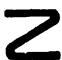
\includegraphics[keepaspectratio]{images/part002_84c4f053.jpg}}


\begin{enumerate}
\def\labelenumi{(\arabic{enumi})}
\setcounter{enumi}{4}
\tightlist
\item
  The powers of any prime ideal are not necessarily primary ideals (Exercise 1). On the other hand, there exist primary ideals which are not powers of prime ideals (Exercise 1).
\end{enumerate}

PROPOSITION 2. Let M be a module over a Noetherian ring A, p a prime ideal of A and \((Q_{i})_{i\in I}\) a non-empty finite family of submodules of M which are p-primary with respect to M. Then \(\bigcap_{i\in I} Q_{i}\) is p-primary with respect to M.

\(\mathrm{M}/\left(\bigcap_{i\in\mathrm{I}}\mathrm{Q}_{i}\right)\) is isomorphic to a submodule \(\neq0\) of the direct sum \(\bigoplus_{i\in\mathrm{I}}(\mathrm{M}/\mathrm{Q}_{i})\) . Now

\[
\operatorname{Ass} \left(\bigoplus_ {i \in I} (M / Q _ {i})\right) = \bigcup_ {i \in I} \operatorname{Ass} (M / Q _ {i}) = \{p \}
\]

(§ 1, no. 1, Corollary 1 to Proposition 3). Hence \(\operatorname{Ass}\left(M / \left(\bigcap_{i \in I} Q_i\right)\right) = \{p\}\) (§ 1, no. 1, Proposition 3 and Corollary 1 to Proposition 2).

PROPOSITION 3. Let A be a Noetherian ring, S a multiplicative subset of A, p a prime ideal of A, M an A-module, N a submodule of M and \(i = i_{A}^{S}\) the canonical mapping of M to \(S^{-1}M\) .

\begin{enumerate}
\def\labelenumi{(\roman{enumi})}
\item
  Suppose that \(\mathfrak{p} \cap \mathbf{S} \neq \varnothing\) . If \(\mathbf{N}\) is \(\mathfrak{p}\) -primary with respect to \(\mathbf{M}\) , then \(\mathbf{S}^{-1}\mathbf{N} = \mathbf{S}^{-1}\mathbf{M}\) .
\item
  Suppose that \(\mathfrak{p} \cap \mathbf{S} = \varnothing\) . For \(\mathbf{N}\) to be \(\mathfrak{p}\) -primary with respect to \(\mathbf{M}\) , it is necessary and sufficient that \(\mathbf{N}\) be of the form \(i^{-1}(\mathbf{N}')\) , where \(\mathbf{N}'\) is a sub- \(\mathbf{S}^{-1}\mathbf{A}\) -module of \(\mathbf{S}^{-1}\mathbf{M}\) which is \((\mathbf{S}^{-1}\mathfrak{p})\) -primary with respect to \(\mathbf{S}^{-1}\mathbf{M}\) ; then \(\mathbf{N}' = \mathbf{S}^{-1}\mathbf{N}\) .
\item
  If \(\mathfrak{p} \cap S \neq \varnothing\) and \(N\) is \(\mathfrak{p}\) -primary with respect to \(M\) , then
\end{enumerate}

\[
\mathrm{Ass} _ {\mathbf {S} ^ {- 1} \mathbf {A}} (\mathrm{S} ^ {- 1} (\mathrm{M} / \mathrm{N})) = \varnothing
\]

(§ 1, no. 2, Corollary to Proposition 5) and hence \(S^{-1}(M/N) = 0\) (§ 1, no. 1, Corollary 1 to Proposition 2), whence \(S^{-1}M/S^{-1}N = 0\) .

\begin{enumerate}
\def\labelenumi{(\roman{enumi})}
\setcounter{enumi}{1}
\tightlist
\item
  Suppose that \(\mathfrak{p} \cap \mathrm{S} = \varnothing\) . If \(\mathbf{N}\) is \(\mathfrak{p}\) -primary with respect to \(\mathbf{M}\) , then \(\operatorname{Ass}_{\mathbf{S}^{-1}\mathbf{A}}(\mathrm{S}^{-1}(\mathrm{M/N})) = \{\mathrm{S}^{-1}\mathfrak{p}\}\) ( \(\S 1\) , no. 2, Corollary to Proposition 5) and hence the submodule \(\mathbf{N}' = \mathrm{S}^{-1}\mathbf{N}\) of \(\mathrm{S}^{-1}\mathbf{M}\) is \((\mathrm{S}^{-1}\mathfrak{p})\) -primary; moreover, if \(s \in \mathbf{S}\) and \(m \in \mathbf{M}\) are such that \(sm \in \mathbf{N}\) , then \(m \in \mathbf{N}\) , for the homothety with ratio \(s\) in \(\mathbf{M/N}\) is injective, whence \(\mathbf{N} = \overline{i}^{1}(\mathbf{N}')\) (Chapter II, \(\S 2\) , no. 4, Proposition 10). Conversely, let \(\mathbf{N}'\) be a submodule of \(\mathrm{S}^{-1}\mathbf{M}\) which is \((\mathrm{S}^{-1}\mathfrak{p})\) -primary with respect to \(\mathrm{S}^{-1}\mathbf{M}\) ; let us write \(\mathbf{N} = \overline{i}^{1}(\mathbf{N}')\) ; then \(\mathbf{N}' = \mathrm{S}^{-1}\mathbf{N}\) (Chapter II, \(\S 2\) , no. 4, Proposition 10) and \(\operatorname{Ass}_{\mathbf{S}^{-1}\mathbf{A}}(\mathrm{S}^{-1}(\mathrm{M/N})) = \operatorname{Ass}_{\mathbf{S}^{-1}\mathbf{A}}((\mathrm{S}^{-1}\mathbf{M})/\mathrm{N}') = \{\mathrm{S}^{-1}\mathfrak{p}\}\) . As the canonical mapping \(\mathrm{M/N} \to \mathrm{S}^{-1}(\mathrm{M/N})\) is injective, no prime ideal of \(\mathbf{A}\) associated with \(\mathbf{M/N}\) meets \(\mathbf{S}\) ( \(\S 1\) , no. 2, Proposition 6); it follows that \(\operatorname{Ass}(\mathrm{M/N}) = \{\mathfrak{p}\}\) ( \(\S 1\) , no. 2, Corollary to Proposition 5), so that \(\mathbf{N}\) is \(\mathfrak{p}\) -primary with respect to \(\mathbf{M}\) .
\end{enumerate}

